\documentclass[10pt,a4paper]{article}
\usepackage{caratula}
\usepackage{geometry}
\renewcommand\familydefault{\sfdefault} % Default family: serif 
\usepackage[usenames,dvipsnames]{xcolor}
\usepackage{tikz}
\usepackage{soul}
\usetikzlibrary{calc} 
\usetikzlibrary{arrows, decorations.markings,positioning,backgrounds,shapes}
\definecolor{EMP}{HTML}{77DD77} % Green1
\definecolor{NOR}{HTML}{06500C} % Green2
\usepackage{ulem}
\renewcommand{\ULdepth}{3pt}
\usepackage{tikz-dependency}
\usepackage{graphicx} 
\usepackage{indentfirst}
\setlength{\parindent}{12pt}

%\usetikzlibrary{positioning}




\titulo{TP1 }
\subtitulo{Relación PBI - Cantidad de sedes Argentinas en el exterior}

\fecha{\today}

\materia{Laboratorio de Datos}
\grupo{GRUPO 100}

\integrante{Chapana Puma, Joselin Miriam}{1197/21}{yoselin.chapana@gmail.com}
\integrante{Martinelli, Lorenzo}{364/23}{martinelli.lorenzo12@gmail.com}
\integrante{Padilla, Ramiro Martin}{1636/21}{ramiromdq123@gmail.com}

\graphicspath{{../static/}}


\begin{document}
\newgeometry{margin=2cm}

\maketitle

\restoregeometry
%\newgeometry{top=3cm,bottom=3cm,right=3cm,left=3cm} para editar margenes menos del titulo 


\section{Resumen}
este es el resumen


\section{Introducción} \vspace{0.1cm}

\subsection{Objetivo y Fuente} \vspace{0.1cm}

El objetivo principal de este trabajo es encontrar una relación entre la cantidad de sedes de Argentina en un país y su PBI, para esto, trabajaremos con los siguientes datos, 

\begin{itemize}
	\item PBI per cápita de los paises (1)
	\item Representaciones Argentinas en el exterior, donde tenemos, Datos básicos de las sedes, Datos completos de sedes y secciones (2)
\end{itemize}

\noindent (1) https://data.worldbank.org/indicator/NY.GDP.PCAP.CD \vspace {0.1cm}

\noindent (2) https://datos.gob.ar/dataset/exterior-representaciones-argentinas \vspace{0.1cm}
 
\subsection{Procedimiento}

\indent Este trabajo tendrá varias etapas, comenzando con el planteo de un Diagrama de Entidad Relacional (DER) adecuado al objetivo de nuestro trabajo, continuando con la elaboración y normalización de un Modelo Relacional. Además, de llevar a cabo una limpieza de los datos utlizando ciertas metricas, en particular, utilizaremos el método GQM. \par

Una vez tengamos los datos limpios y el modelo normalizado, pasaremos al procesamiento y visualización de datos en Python utilizando librerias como Pandas, Inlinesql, Matplotlib entre otras con el fin de elaborar nuestras conclusiones, ¿Será mayor el PBI de aquellos paises con sedes Argentinas? ¿Influirá la cantidad de sedes y/o secciones de estas?.  

\section{Procesamiento de Datos} \vspace{0.2cm}

\subsection{Diagrama de Entidad Relacional} \vspace{0.2cm}

A continuación, el DER con la información necesaria para cumplir el objetivo \vspace{0.2cm}

\begin{figure}[ht]
	\centering
	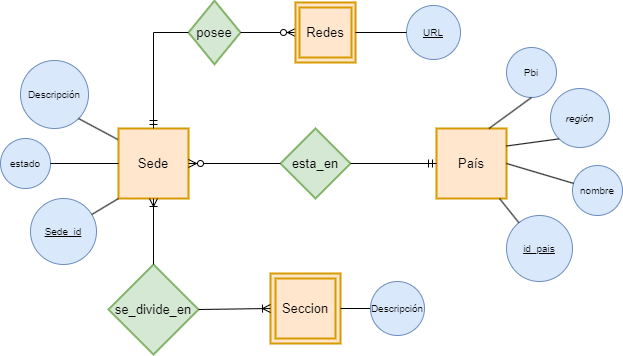
\includegraphics[width=1.1\textwidth]{DERPBI.png}
	\caption{Diagrama de Entidad Relacional}
	\label{fig:ejemplo}
\end{figure}




\newbox\ubox

\begin{tikzpicture}[
    EMP/.style={% Style for empatized boxes
        rectangle, line width =1pt,
        anchor=west,
        underline, % new property
        align=center,
        text=Black,
        minimum height=.8cm,
        text height=1.7ex,
            text depth=.25ex,
        fill=EMP,
        draw=black,
        },
    NOR/.style={% Style for normal boxes.
        rectangle, 
        line width =1pt,
        anchor=west,
        align=left,
        minimum height=.6cm,
        text height=1.5ex,
            text depth=.25ex,
            text=white,
        fill=NOR,
        draw=black,
        inner ysep=5pt
        },
    underline/.append style={% define new style property
        execute at begin node={%
            \setbox\ubox=\hbox\bgroup
            },
            execute at end node={%
                \egroup\uline{\box\ubox}%
                }
             },
    ] % Uff that is all the configuration for tickzpicture xD

% Define an brute force objet "Frame"
% Variables 1:Position, 2: Identifier, 3: Title of frame 4: Subframe/Boxtype
 \def\Frame(#1)#2[#3]#4{%
  \begin{scope}[shift={(#1)}] 
      \node[font=\bf, anchor=west] (Title) at (-0.2,0.7) {#3}; 
       \edef\k{0}% Variable for box positión
       \edef\x{0}% Variable for named coordinate centering - below box
       \foreach \id/\style in {#4} {%enter sub frame data Name/Boxtype ,Name2/Boxtype | An space before Boxtype is needed 
            \node[\style] (h) at (\k pt,0) {\id}; %  % Draw a node depending on the variables.
            \pgfmathparse{\k+0.5*width{"\id"}+3.4pt} % Uses the textwidth to calculate named coordinate  
            \xdef\x{\pgfmathresult} % The resul is saved in the variable \x
            \draw (\x pt,-0.4) coordinate (\id#2); %Create a named coordinate concatenated: "sub frame data Name"+"identifier"
            \pgfmathparse{\k+width{"\id"}+6.8pt}% Calculate positión for each subframe box.       
        \xdef\k{\pgfmathresult}% Save the value to be added to the next iteration value.
       }    
  \end{scope}
}% disadvantages: Is not posible to use Frame data Name like: Name_another_desc instead I use Name-another-desc

% Start drawing
% \node[EMP node] (dm) at (0,0) {{Sometext/EMP,another/EMP}};
  \Frame(0,0){3}[PAIS]{
    IdPais/EMP,
    NombrePais/NOR};

 \Frame(0,-2.5){1}[SEDE]{%first frame identified as 1 named EMPLOYEE
    IdSede/EMP,% see that it is necessary to add a space
    IdPais/NOR,
    Descripción/NOR,
    Estado/NOR}; 

 \Frame(0,-5){2}[REDES]{
    IdSede/EMP,
    Urls/EMP};  

 \Frame(0,-7.5){4}[REGION]{
    IdPais/EMP,
    Region/NOR};

  \Frame(0,-10){5}[SECCIONES]{
    IdSede/EMP,
    SeccionDescripcion/EMP};     

 \Frame(0,-12.5){6}[PBI]{
    IdPais/EMP,
    PBI-2022/NOR,}; 

% Start drawing arrows:
% In this part I use the named coordinates to draw the arrows.
    \draw[thick,<-,thick,>=latex] % From Essn6 to Ssn1  
        (IdSede1)++(0.1,0) -- ++(0,-.55) -- ++(4.5,0) coordinate (inter) %inter is the name of coordinate register
        -- (IdSede2 -| inter) -- ++(0,-0.4) coordinate (inter)  % to calculate intersections.
        -- (IdSede2 |- inter) --++(0,0.4); %
        
    \draw[thick,<-,thick,>=latex]
        (IdPais3) -- ++(0,-.675) -- ++(5.2,0) coordinate (inter) 
        -- (IdPais4 -| inter) -- ++(0,-0.2) coordinate (inter) 
        -- (IdPais4 |- inter) --++(0,0.2); %

     \draw[thick,<-,thick,>=latex]
        (IdSede1)++(-0.3,0) -- ++(0,-.85) -- ++(4.3,0) coordinate (inter) 
        -- (IdSede5 -| inter) -- ++(0,-0.2) coordinate (inter) 
        -- (IdSede5|- inter) --++(0,0.2); %.
        
     \draw[thick,<-,thick,>=latex]
        (IdSede1)++(-0.3,0) -- ++(0,-.85) -- ++(4.3,0) coordinate (inter) 
        -- (IdSede5 -| inter) -- ++(0,-0.2) coordinate (inter) 
        -- (IdSede5|- inter) --++(0,0.2); %.

    \draw[thick,<-,thick,>=latex] % From Essn6 to Ssn1  
        (IdPais3)++(0.2,0) -- ++(0,-.5) -- ++(5.2,0) coordinate (inter) %inter is the name of coordinate register
        -- (IdPais1 -| inter) -- ++(0,-0.4) coordinate (inter)  % to calculate intersections.
        -- (IdPais1 |- inter) --++(0,0.45); %

    \draw[thick,<-,thick,>=latex] % From Essn6 to Ssn1  
        (IdPais3)++(-0.2,0) -- ++(0,-.85) -- ++(5.8,0) coordinate (inter) %inter is the name of coordinate register
        -- (IdPais6 -| inter) -- ++(0,-0.4) coordinate (inter)  % to calculate intersections.
        -- (IdPais6 |- inter) --++(0,0.45); %

        
\end{tikzpicture}

\section{Decisiones tomadas}


\section{Análisis de datos}


\section{Conclusiones}

\end{document}